\subsection{Polarization}

A beam of light can be described as a plane electromagnetic wave, like so:
$$\vec E(z,t)=E_0\cdot\hat e_x\cdot e^{i(\omega t-kz)}$$
$$\vec B(z,t)=B_0\cdot\hat e_y\cdot e^{i(\omega t-kz)}$$
The propagation vector $\hat e_z$ together with $\vec E$ and $\vec B$ create 
an orthogonal system. \\ \\ The direction of $\vec E$ defines the polarization, 
which can be distinguished into three types:
\begin{enumerate}
    \item linear polarization
    \item elliptical polarization
    \item circular polarization
\end{enumerate}
If the wave is thought of as a superposition of two orthogonal plane waves,
elliptical polarization occurs when the phase difference of those two waves
is exactly $\Delta\varphi=\frac{\pi}{2}$. If, in addition, both waves
carry the same amplitude, we speak of circular polarization.
\textcolor{red}{What happens for $\Delta\varphi\neq\frac{\pi}{2}$?}

\subsubsection{Snell's law}
If a beam of light reaches the surface between two optical media with
refractive indices $n_1$ and $n_2$, the beam splits into a reflected and a
refracted one. The refraction angle $\alpha_2$ can be determined by
$$n_1\cdot sin(\alpha_1)=n_2\cdot sin(\alpha_2)$$
The angles $\alpha_1$ and $\alpha_2$ are taken between the
incoming/outgoing beam of light and the surface. \\ \\ For reflection,
the condition $\alpha_{in}=\alpha_{out}$ must hold.

\subsubsection{Malus law}
The Malus law states that when a perfect polarizer is placed in a polarized
beam of light, the intensities before and after tranversing the polarizer
are related by
$$I_f=I_i\cdot cos^2(\theta)$$
Here, $\theta$ is the angle between the light's initial polarization
direction and the axis of the polarizer.

\subsubsection{Brewster's angle}
Brewster's angle is a specific angle of incidence at which light with a
particular polarization is perfectly transmitted through a transparent
dielectric surface, without any reflection. \\ \\ When unpolarized light
is incident at this angle, the light that is reflected from the surface is
therefore perfectly polarized. \textcolor{red}{Meaning? Sources?}

\subsubsection{Fresnel equations}
The Fresnel equations describe the reflection and transmission of light
when incident on an interface between different optical media.
\textcolor{red}{equations}

\subsubsection{Reflection and polarization}
From Maxwell's equation the amplitudes and intensities of the two beams
can be derived. The amplitude coefficients corresponding to the reflected and
the transmitted beams are labeled $r$ and $t$. The intensity coefficients
$R$ and $T$ can easily be calculated by taking the square of $r$ and $t$.
If the polarization is perpendicular to the plane of incidence
(transversal-electric, S-polarization), the coefficients are given by
$$r_{TE}=-\frac{sin(\alpha_1-\alpha_2)}{sin(\alpha_1+\alpha_2)}$$
\begin{center}and\end{center} $$t_{TE}=\frac{2\cdot sin(\alpha_1)\cdot
cos(\alpha_2)}{sin(\alpha_1+\alpha_2)}$$
If the wave is polarized parallel to the plane of incidence, we speak of
transversal-magnetic polarization (German: P-Polarisation), the coefficients
are given by
$$r_{TM}=\frac{tan(\alpha_1-\alpha_2)}{tan(\alpha_1+\alpha_2)}$$
\begin{center}and\end{center} $$t_{TM}=\frac{2\cdot sin(\alpha_1)\cdot
 cos(\alpha_2)}{sin(\alpha_1+\alpha_2)\cdot
cos(\alpha_1-\alpha_2)}$$

\subsubsection{Birefringence}

\subsubsection{Wave plates}


\newpage
\subsection{Electro-optical effect}
Some materials experience a change in their optical properties when they are
brought into an external electric field. If the refractive index $n$ is a
function of the applied field $E$, we speak of an electro-optical modulator
(EOM).

\subsubsection{Pockels effect}
The refractive index $n=n(E)$ can be expanded around $E=0$
for small field strengths. \\ \\ With
$r=-\frac{2}{n^3}\bigg(\frac{dn}{dE}\bigg)\bigg|_{E=0}$ and
$s=-\frac{1}{n^3}\bigg(\frac{d^2n}{dE^2}\bigg)\bigg|_{E=0}$,
this leads to the relation
$$n(E)=n_0-\frac{1}{2}rn^3E-\frac{1}{2}sn^3E^2$$
The linear electro-optical effect, also called Pockels effect,
occurs for $r\gg s$:
$$n(E)\approx n_0-\frac{1}{2}rn^3E$$
Here, $r$ is called the Pockels coefficient. If, on the other hand, $r\ll s$,
the quadratic dependence of $n$ on $E$ is known as the Kerr effect.
This effect will not be studied in this lab course.

\subsubsection{Pockels effect in a non-isotropic crystal}
Since the electro-optical crystals are in general birefringent, the
Pockels coefficient is not a scalar, but a tensor. For the material
LiNbO$_3$, the entries of this coefficient-tensor are given by
$$\begin{pmatrix}
    r_{11} & r_{12} & r_{13} \\
    r_{21} & r_{22} & r_{23} \\
    r_{31} & r_{32} & r_{33} \\
    r_{41} & r_{42} & r_{43} \\
    r_{51} & r_{52} & r_{53} \\
    r_{61} & r_{62} & r_{63}
\end{pmatrix}=\begin{pmatrix}
    0 & -r_{22} & r_{13} \\
    0 & r_{22} & r_{13} \\
    0 & 0 & r_{33} \\
    0 & r_{51} & 0 \\
    r_{51} & 0 & 0 \\
    -r_{22} & 0 & 0 \\
\end{pmatrix}=\begin{pmatrix}
    0 & -3.4 & 8.6 \\
    0 & 3.4 & 8.6 \\
    0 & 0 & 30.8 \\
    0 & 28 & 0 \\
    28 & 0 & 0 \\
    -3.4 & 0 & 0
\end{pmatrix}\cdot 10^{-12}\ \frac{\textnormal{m}}{\textnormal{V}}$$


\newpage
\subsection{Acousto-optical effect}
If a sound wave passes through a crystal, its density varies periodically,
which also leads to a periodic variation in the refractive index.
A plane sound wave with wavelength $\lambda_s$ in a crystal with
initial refractive index $n_0$ can be described by
$$n(x,t)=n_0-\Delta n\cdot cos\bigg(\omega t-\frac{2\pi}{\lambda_s}x\bigg)$$
Here, the amplitude $\Delta n=\frac{1}{2}pn^3s_0$ depends on the
photo-elastic constant $p$ and the amplitude of the strain $s_0$.
The interaction between laser beam and sound wave occurs either as Bragg
diffraction for long interaction lengths or as the Debye-Sears effect
for short interaction lengths, i.e. for a thin crystal or thin sound beam.
\begin{figure}[h!]
    \center
    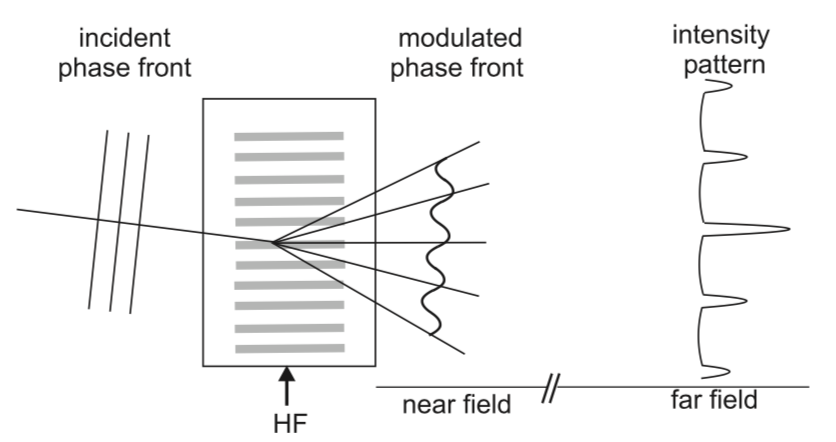
\includegraphics[width=.5\textwidth]{acousto_optical_effect_deformation}
    \caption{deformation of a plane wavefront by a sound wave}
    \label{acousto_optical_effect_deformation}
\end{figure}
Parts of the light beam that are travelling through the denser regions
experience a phase shift. Maxima in the far field can be observed, if
these parts of the beam interfere constructively with each other, as can
be seen in the next figure.
\begin{figure}[h!]
    \center
    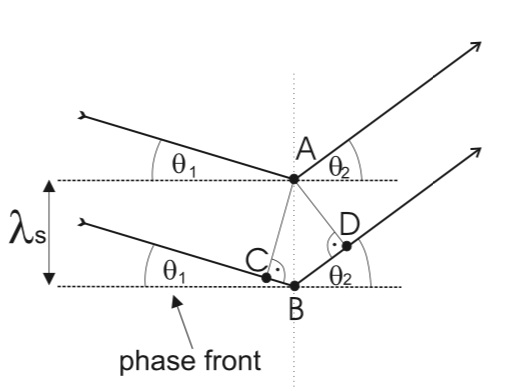
\includegraphics[width=.5\textwidth]{acousto_optical_effect_interference}
    \caption{interference of different sections of the light beam}
    \label{acousto_optical_effect_interference}
\end{figure}
Because the light is interacting with a moving sound wave, the
diffracted light is Doppler-shifted: $$\textcolor{red}{\omega_{out}=
\omega_{in}+m\Delta\omega=\omega_{in}+m\omega_s}$$
\\
A different approach to explain the effect of an AOM on a light beam is to
describe the system as two scattering quasi-particles, namely a phonon
and a photon. Their momentum vectors are $\hbar\vec k_l$ and $\hbar\vec k_s$,
respectively. Conservation of momentum and energy leads to the relations
$$\vec k_{l,f}=\vec k_{l,i}\pm m\vec k_s$$
\begin{center}and\end{center}
$$\nu_{l,f}=\nu_{l,i}\pm m\nu_s$$
Here, $m$ is the diffraction order, i.e. the number of phonons that
interacted with the photon. Constructive interference occurs when
$$sin\theta_1+sin\theta_2=m\frac{\lambda}{\lambda_s}$$
Here, $\theta_1$ is the angle under which light enters the crystal
and $\theta_2$ the diffraction angle.
\textcolor{red}{efficiency}
